\chapter{Risultati}
In questo capitolo saranno presentati i risultati ottenuti nelle varie
simulazioni. Quando non meglio specificato, i parametri sono stati mantenuti
come quelli indicati nel paper. Visto il nostro assegnamento dei valori di
fitness, il punteggio massimo è 100 punti, ottenuto non entrando mai nei muri,
non scontrandosi mai con altri robot e raccogliendo tutte le lattine.

\section{Entità Invisibili - Vista a Croce}
\begin{figure}[ht]
	\centering
	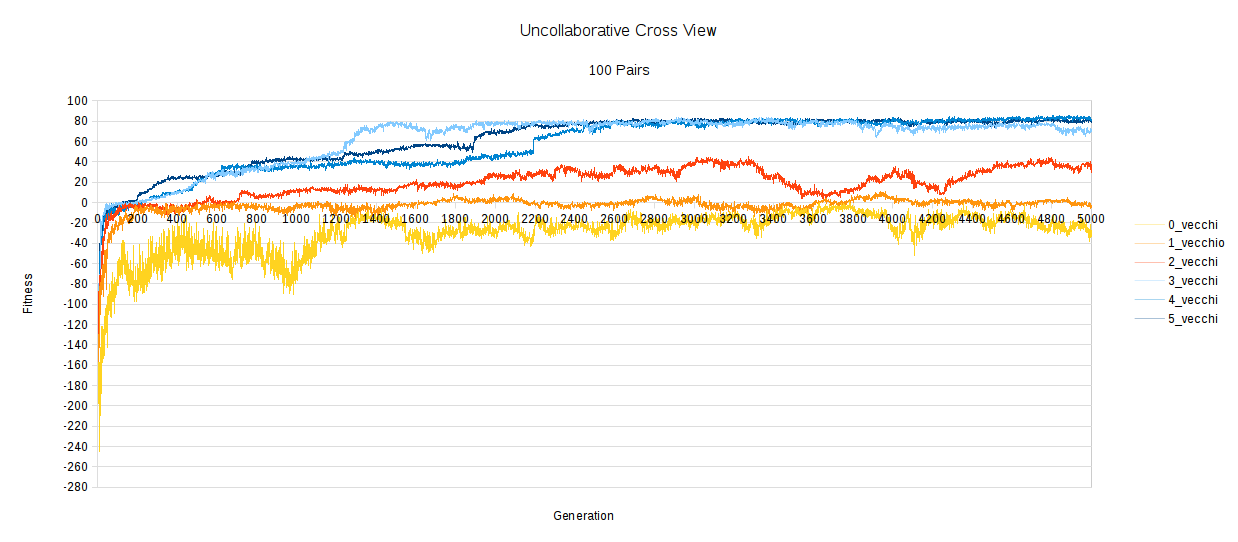
\includegraphics[scale=0.7,angle=90]{imgs/uncollaborative_cross_100_pairs_0_5_vecchi.png}
	\caption{Vista a croce non collaborativa, 100 coppie}
	\label{figure:uncoll_cross_100_0_5}
\end{figure}
\begin{figure}[ht]
	\centering
	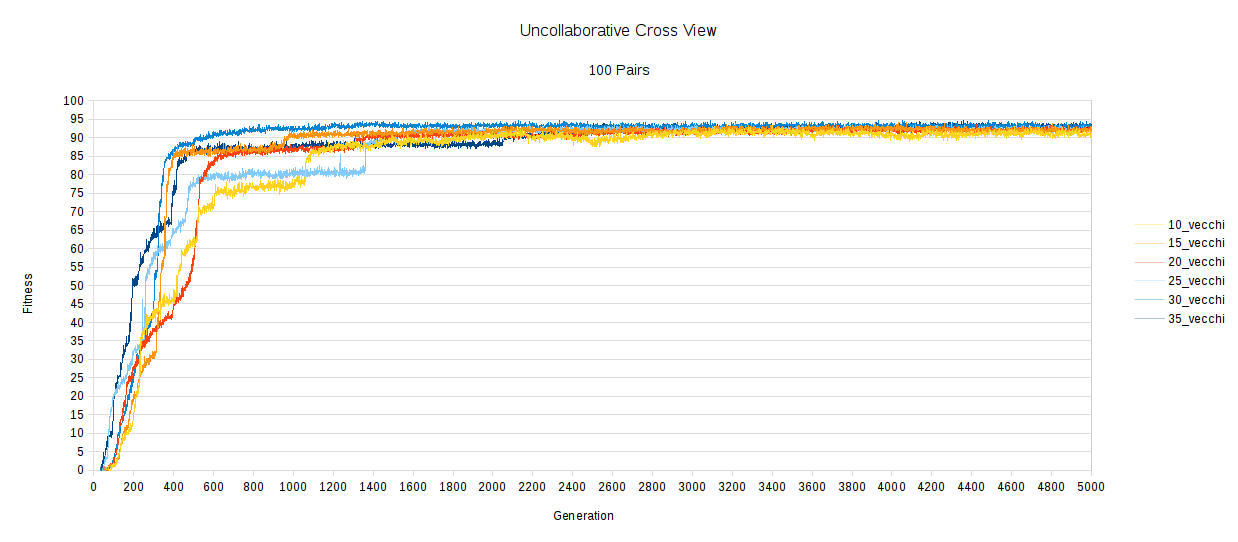
\includegraphics[scale=0.7,angle=90]{imgs/uncollaborative_cross_100_pairs_10_35_vecchi.png}
	\caption{Vista a croce non collaborativa, 100 coppie}
	\label{figure:uncoll_cross_100_10_35}
\end{figure}
\begin{figure}[ht]
	\centering
	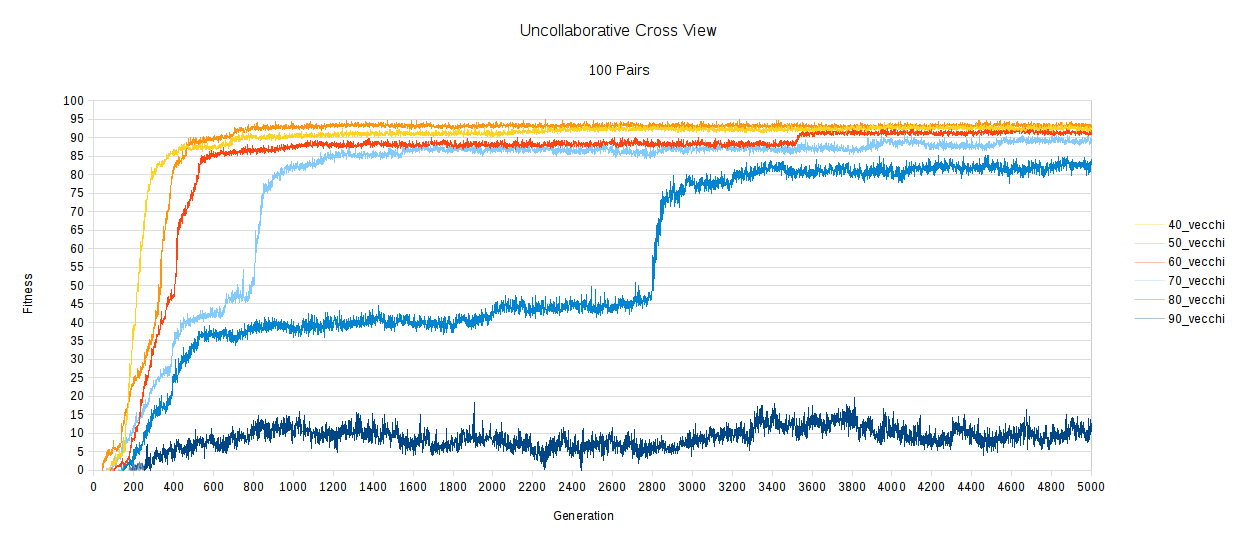
\includegraphics[scale=0.7,angle=90]{imgs/uncollaborative_cross_100_pairs_40_90_vecchi.png}
	\caption{Vista a croce non collaborativa, 100 coppie}
	\label{figure:uncoll_cross_100_40_90}
\end{figure}
\begin{figure}[ht]
	\centering
	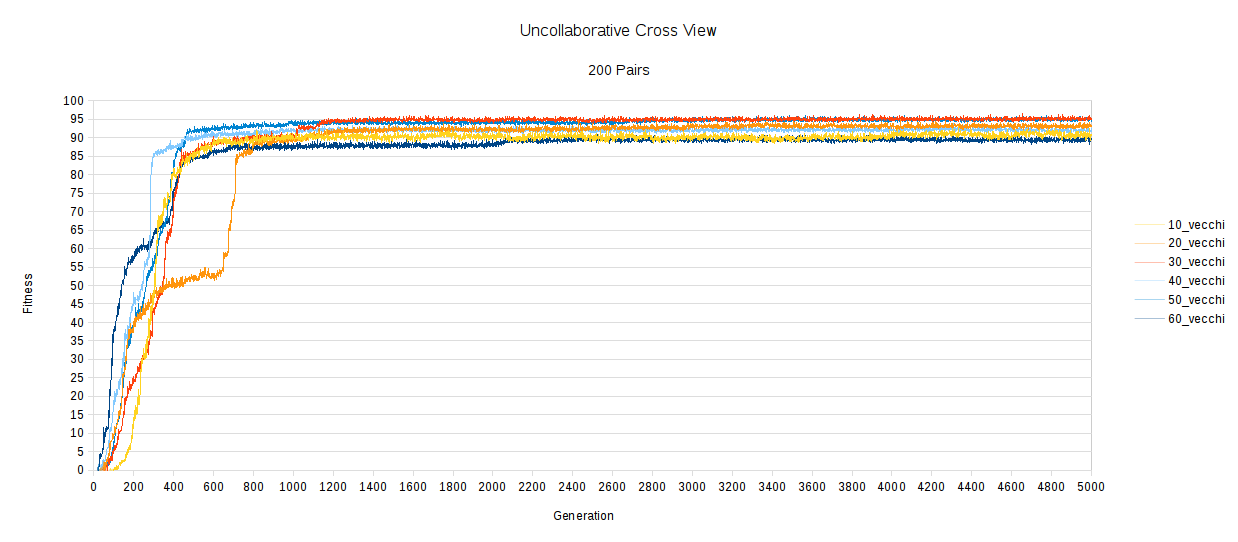
\includegraphics[scale=0.7,angle=90]{imgs/uncollaborative_cross_200_pairs_10_60_vecchi.png}
	\caption{Vista a croce non collaborativa, 200 coppie}
	\label{figure:uncoll_cross_200_10_60}
\end{figure}
\begin{figure}[ht]
	\centering
	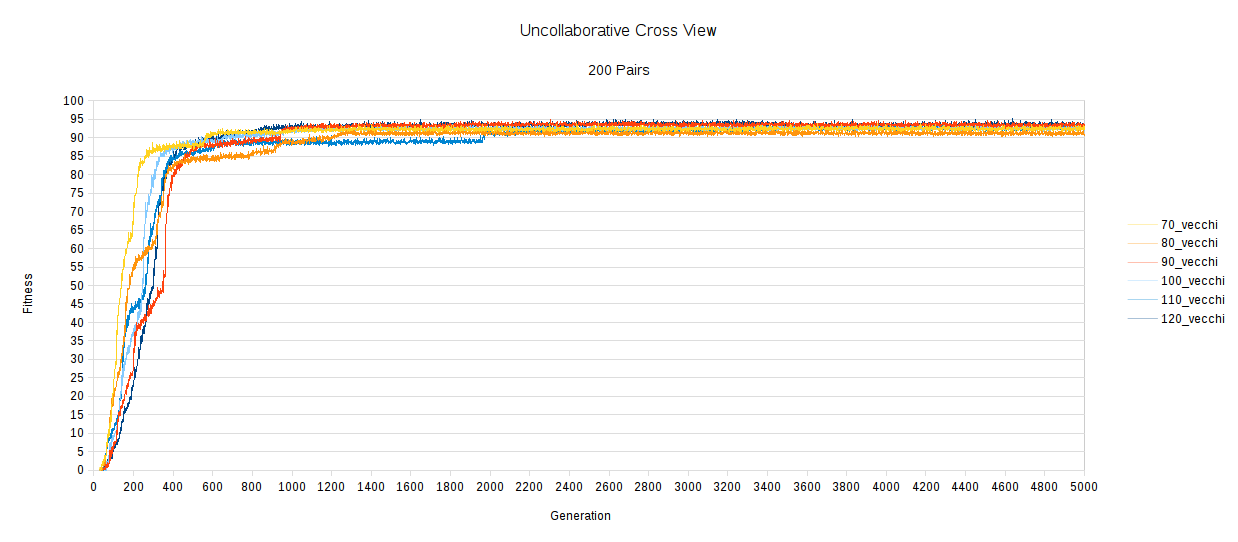
\includegraphics[scale=0.7,angle=90]{imgs/uncollaborative_cross_200_pairs_70_120_vecchi.png}
	\caption{Vista a croce non collaborativa, 200 coppie}
	\label{figure:uncoll_cross_200_70_120}
\end{figure}
\begin{figure}[ht]
	\centering
	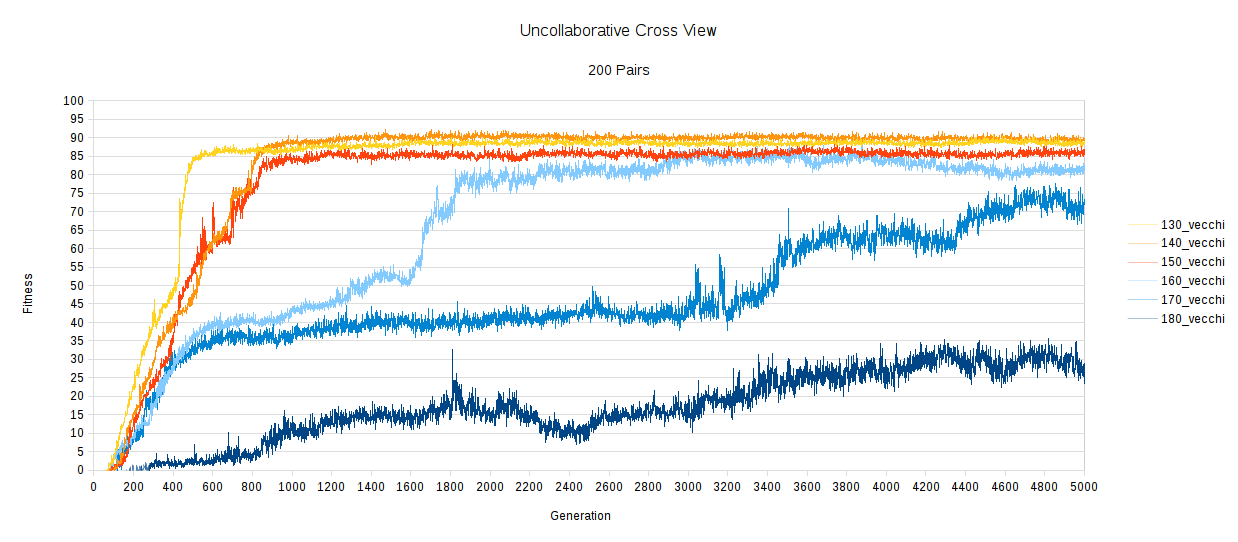
\includegraphics[scale=0.7,angle=90]{imgs/uncollaborative_cross_200_pairs_130_180_vecchi.png}
	\caption{Vista a croce non collaborativa, 200 coppie}
	\label{figure:uncoll_cross_200_130_180}
\end{figure}
\begin{figure}[ht]
	\centering
	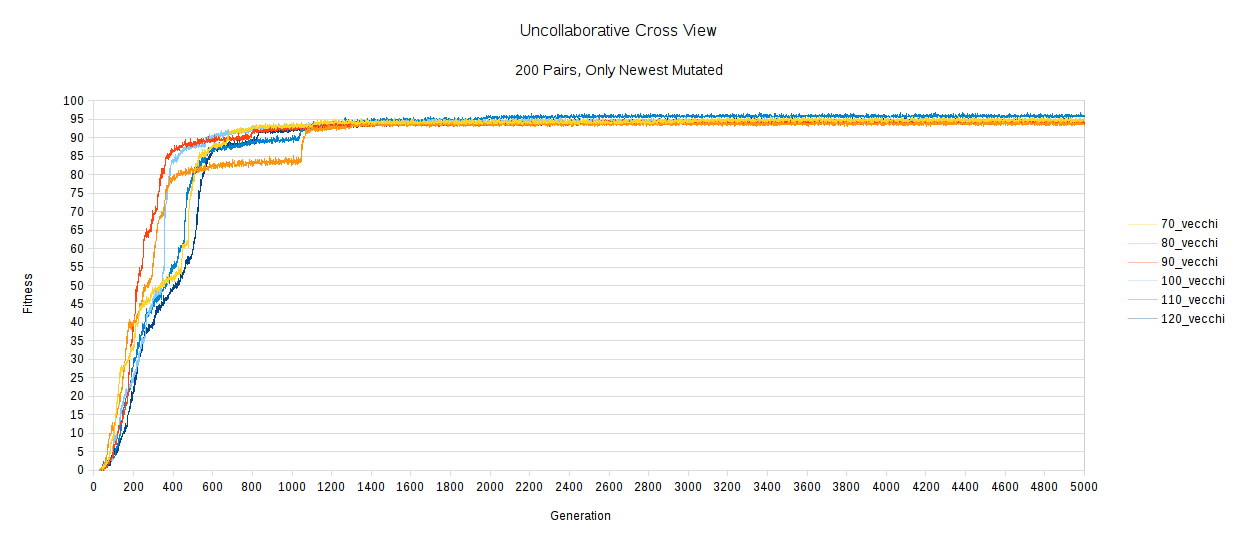
\includegraphics[scale=0.7,angle=90]{imgs/uncollaborative_cross_200_pairs_70_120_vecchi_solo_nuovi_mutati.png}
	\caption{Vista a croce non collaborativa, 200 coppie}
	\label{figure:uncoll_cross_200_70_120_vecchi_non_mutati}
\end{figure}
La prima simulazione è stata effettuata usando lo schema del paper con 100
coppie, ovvero 200 robot. In 5000 generazioni il valore di fitness, dopo un
primo incremento, si è sempre mantenuto attorno al valore 0. Questo ci ha fatto
supporre che la strategia di evoluzione da noi adottata potesse essere errata.
Abbiamo dunque deciso di copiare alcuni degli individui vecchi nella nuova
generazione.\newline
La Figura~\ref{figure:uncoll_cross_100_0_5} mostra i valori di 6 simulazioni
nelle quali abbiamo mantenuto da 0 a 5 coppie (le migliori) dalla vecchia alla
nuova generazione. Come è possibile notare, più sono gli individui che sono
mantenuti invariati e più alto è il valore di fitness raggiunto.\newline
In Figura~\ref{figure:uncoll_cross_100_10_35} abbiamo proseguito con il
ragionamento, copiando nella vecchia generazione da 10 a 35 coppie,
incrementando l'intervallo da 1 a 5. I valori di fitness si mantengono tutti fra
i 90 ed i 95 punti.\newline
A questo punto ci siamo chiesti quando le performance sarebbero crollate ed
abbiamo ulteriormente iterato il procedimento mantenendo da 40 a 90 coppie,
procedendo per intervalli di 10. Come è mostarto in Figura
\ref{figure:uncoll_cross_100_40_90}, man mano che il numero di coppie vecchie è
passato nella nuova generazione, il valore di fitness inizia a scendere, fino
a mostrare cali vertiginosi con 80 e 90 coppie.\newline
Avendo notato come la modifica anche piccola di un semplice parametro (il numero
di coppie vecchie da mantenere nella nuova popolazione) possa influenzare in
maniera significativa l'evoluzione, abbiamo deciso di ripetere lo stesso
procedimento aumentando il numero di coppie da 100 a 200. La Figura
\ref{figure:uncoll_cross_200_10_60} mostra l'andamento dell'evoluzione tenendo
da 10 a 60 coppie, la Figura~\ref{figure:uncoll_cross_200_70_120} da 70 a 120 e,
infine, la Figura~\ref{figure:uncoll_cross_200_130_180} grafica l'andamento dei
valori di fitness tenendo da 130 a 180 coppie.\newline
La differenza fra i valori di fitness raggiunti con 200 coppie rispetto ai
valori raggiunti con 100 coppie non è poi così grande. È però presente una
costante: i valori di fitness più alti sono raggiunti mantenendo una percentuale
di coppie vecchie da una generazione all'altra che va dal 10\% al 60\%.\newline
Abbiamo poi effettuato un'ultima simulazione tenendo i risultati migliori con
200 coppie dove le mutazioni genetiche sono state applicate solo ai nuovi
individui generati e non più anche ai vecchi. I risultati sono riportati in
Figura~\ref{figure:uncoll_cross_200_70_120_vecchi_non_mutati}.
